\documentclass[aps,nofootinbib,onecolumn,groupedaddress,a4paper]{revtex4}

\usepackage{color}
\usepackage{graphicx}
\usepackage[utf8]{inputenc}


\begin{document}

\title{Measurement of Drift Velocity} 

\author{T. Akdogan}
\affiliation{Department of Physics\\
Bogazici University, Istanbul, Turkey}


\date{March 16, 2011}

\begin{abstract}
You should give a summary of everything in the report in a preferably single paragraph as the abstract.
\end{abstract}

\maketitle


\section{Introduction}
Here, a brief theoretical background of the experiment and its importance to the modern physics must be given.

\section{Experimental Setup}
The method used for the experiment including the experimental setup should be given in this section.

\section{Data and Analysis}
The raw data and methods used to extract the final results must be given in this section. The raw data is shown in Table \ref{rawdata}.
\begin{table}[htdp]
\caption{The raw data taken and the associated error.\label{rawdata}}
\centering
\begin{tabular}{ccc}
\\
$t$ (sec) & $\lambda$ (m) & $\sigma_t$ (sec) \\
\hline
0.0 &  5.15  &  0.244 \\
1.2 &  2.53  &  0.105 \\
2.4 &  0.18  &  0.181 \\
3.6 & -2.07  &  0.272 \\
4.8 & -4.43  &  0.264 \\
6.0 & -7.11  &  0.167 
\end{tabular}
\label{default}
\end{table}%

The raw data is shown in Fig. \ref{rawplot} with blue data points.
\begin{figure}[h]
\caption{My cute figure.\label{rawplot}}
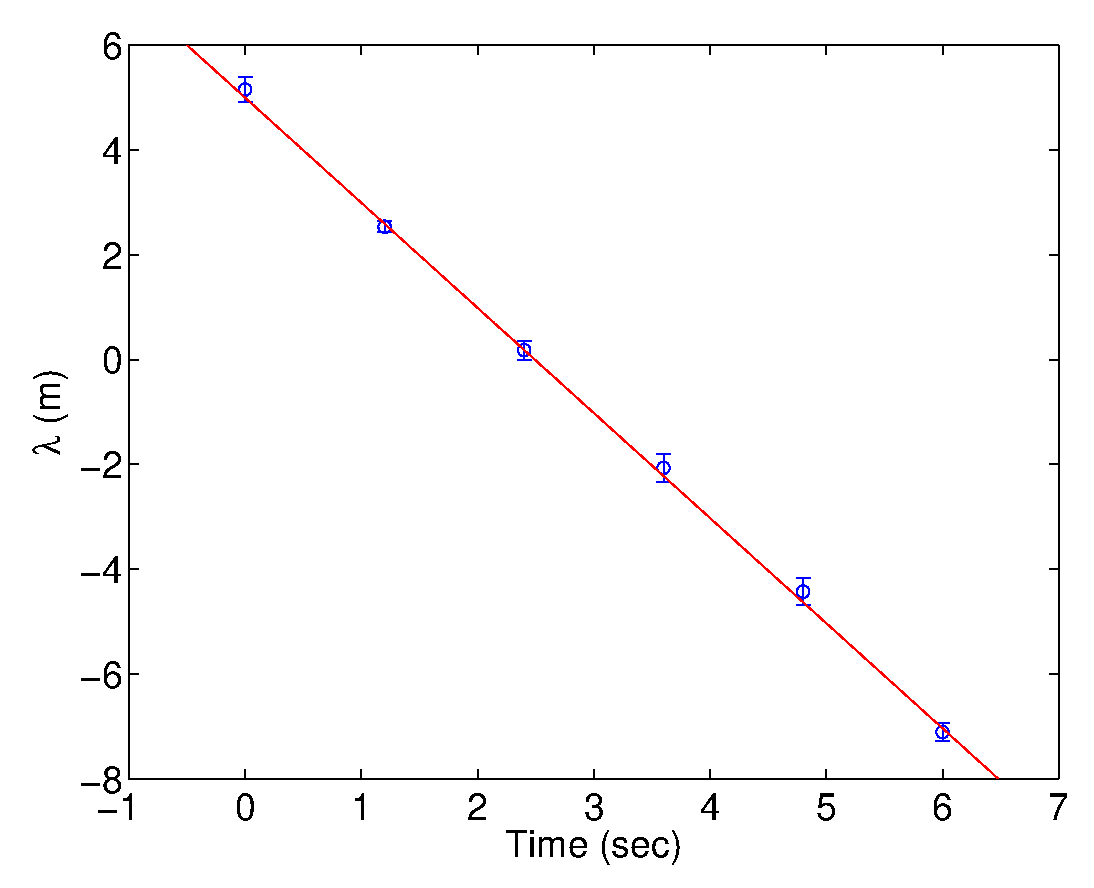
\includegraphics[width=0.5\columnwidth]{sample_plot.eps}
\end{figure}
We fit this data to a straight line with $\lambda = \lambda_o - v t$, and found the follow fit parameters:
\[
\lambda_o = 4.995 \pm 0.115 \mbox{ m } \,\,\,\, , \,\,\,\, v = 2.006 \pm 0.036 \mbox{ m/s }
\]
See Appendix \ref{app_calc} for details.

\section{Results}
A conclusion must be provided here. You should also discuss the results you found in the this section. If you encounter any problem, inaccuracies, etc. this should be discussed as well. Recommendation to improve the experiments, if any, must also be provided.


\begin{acknowledgements}
Acknowledgements belong here. If you received any help from your fellows or professors related to this study, you should express your thanks by citing the kind of help you received. Example: We would like to thank Albert Einstein for his insightful discussion about the theory of photoelectric effect.
\end{acknowledgements}

\appendix
\section{Line Fitting \label{app_calc}}
Here you show the {\bf details} of your calculations. If you wrote any code to analyze your data or did some more complex calculation than required, it must be placed as an appendix.

Here, let us fit our data to $y = n + mx$, keeping in mind that $\lambda_o = n$ and $v = -m$. Then, the relevant sums are shown below:
\begin{eqnarray*}
S & = & \sum \frac{1}{\sigma_i^2} = 201.88 \\
S_x & = & \sum \frac{t_i}{\sigma_i^2} = 515.61 \\
S_y & = & \sum \frac{\lambda_i}{\sigma_i^2} = -25.7018 \\
S_{xy} & = & \sum \frac{t_i \lambda_i}{\sigma_i^2} = -1.6516\times10^3 \\
S_{xx} & = & \sum \frac{t_i^2}{\sigma_i^2} = 2.1076\times10^3
\end{eqnarray*}
Then, we calculate $\Delta$ as:
\[ \Delta = S S_{xx} - S_x^2 = 1.5965\times10^5 \]
Accordingly, we calculate the fit parameters. The interception is at
\[ n = \frac{S_{xx} S_y - S_x S_{xy}}{\Delta} = 4.9948 \]
its error was found:
\[ \sigma_n = \lambda_o = \sqrt{Sxx / \Delta} =  0.1149. \]
The slope is
\[
m = -v = \frac{S S_{xy} - S_x S_y}{\Delta} = -2.0056, \]
and its error is
\[ \sigma_v = \sqrt{S / \Delta} = 0.0356. \]
The red line shown in Fig. \ref{rawplot} show the $\lambda = \lambda_o - vx$ line with the parameters found here.

\end{document}
